\documentclass[11pt]{article}
\usepackage[hmargin=1in,vmargin=1in]{geometry}
\usepackage{xcolor}
\usepackage{amsmath,amssymb,amsfonts,url,sectsty,framed,tcolorbox,framed}
\newcommand{\pf}{{\bf Proof: }}
\newtheorem{theorem}{Theorem}
\newtheorem{lemma}{Lemma}
\newtheorem{proposition}{Proposition}
\newtheorem{definition}{Definition}
\newtheorem{remark}{Remark}
\newcommand{\qed}{\hfill \rule{2mm}{2mm}}
\newtheorem{example}{Example}
\usepackage{tikz}
\usepackage{bm}

\begin{document}
%%%%%%%%%%%%%%%%%%%%%%%%%%%%%%%%%%%%%%%%%%%%%%%%%%%%%%%%%%%%%%%%%%%%%
\noindent
\rule{\textwidth}{1pt}
\begin{center}
{\bf [CS304] Introduction to Cryptography and Network Security}
\end{center}
Course Instructor: Dr. Dibyendu Roy \hfill Winter 2023-2024\\
Scribed by: Raghav Agiwal (202151124) \hfill Lecture (Week 5)
\\
\rule{\textwidth}{1pt}
%%%%%%%%%%%%%%%%%%%%%%%%%%%%%%%%%%%%%%%%%%%%%%%s%%%%%%%%%%%%
%write here



\section*{AES - Advanced Encryption Standard}

AES stands for Advanced Encryption Standard. It's a widely used symmetric encryption algorithm that ensures secure communication and data protection. AES was established as a standard by the U.S. National Institute of Standards and Technology (NIST) in 2001 and has since become one of the most commonly used encryption methods worldwide.

AES operates on fixed-size blocks of data and uses a fixed-length key for encryption and decryption. It supports key sizes of 128, 192, and 256 bits. The number in AES (e.g., AES-128, AES-192, AES-256) refers to the key size in bits.




\subsection*{Key Sizes}

\begin{itemize}
    \item \textbf{AES-128}: Uses a 128-bit key for encryption and decryption. Operates on data blocks of 128 bits and performs 10 rounds of encryption for a given key.
    \item \textbf{AES-192}: Uses a 192-bit key for encryption and decryption. Operates on data blocks of 128 bits and performs 12 rounds of encryption for a given key.
    \item \textbf{AES-256}: Employs a 256-bit key for encryption and decryption. Similar to AES-128, it operates on data blocks of 128 bits but performs 14 rounds of encryption for a given key.
\end{itemize}

\begin{figure}[htbp]
  \centering
  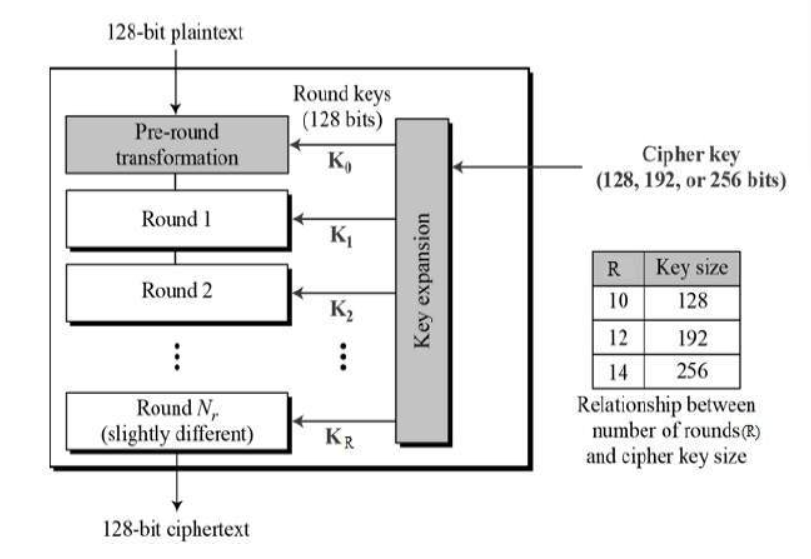
\includegraphics[width=1.00\textwidth]{image4.1.PNG} % Replace example-image with your image file
\end{figure}

\section*{Round functions of AES}
The round function of AES is a crucial component responsible for transforming the input data in a series of steps to enhance its security. It involves several operations performed in a specific sequence:

\begin{enumerate}
    \item \textbf{SubByte}: This operation substitutes each byte in the input with a corresponding byte from a predefined substitution table. It's like swapping each letter in a message with another according to a secret code.
    
    \item \textbf{ShiftRow}: Here, the rows of the input state matrix are shifted by different offsets. It's like reorganizing the rows of a table by moving each row a certain number of positions to the left or right.
    
    \item \textbf{MixColumn}: This is a mathematical operation that operates on the columns of the state matrix. It mixes the bytes within each column to spread out the influence of individual bytes throughout the matrix, enhancing the complexity of the encryption process.
\end{enumerate}


\section{Sub Bytes}

Subbytes is a bijective mapping from 128-bit to 128-bit. 

The input $S$ to subbytes function is a 128-bit binary input. A $4 \times 4$ matrix can be constructed from the input in the following way:

\[ S \rightarrow \begin{bmatrix} S_{00} & S_{01} & S_{02} & S_{03} \\ S_{10} & S_{11} & S_{12} & S_{13} \\ S_{20} & S_{21} & S_{22} & S_{23} \\ S_{30} & S_{31} & S_{32} & S_{33} \end{bmatrix} \]

where $S_{ij}$ is a byte (8-bits). Consider the 128-bit plaintext of 128-bit. The plaintext again can be written as a $4 \times 4$ matrix in the following way:

\[ P = P_0P_1P_2....P_{15}, \text{length of each } P_i \text{ is 8-bit} \]
\[ P \rightarrow \begin{bmatrix} P_0 & P_4 & P_8 & P_{12} \\ P_1 & P_5 & P_9 & P_{13} \\ P_2 & P_6 & P_{10} & P_{14} \\ P_3 & P_7 & P_{11} & P_{15} \end{bmatrix} \]

Similarly, the first round key $K1$ can also be written as a matrix.

\[ K1 = K_0K_1K_2....K_{15}, \text{ length of each } K_i \text{ is 8-bit} \]
\[ K1 \rightarrow \begin{bmatrix} K_0 & K_4 & K_8 & K_{12} \\ K_1 & K_5 & K_9 & K_{13} \\ K_2 & K_6 & K_{10} & K_{14} \\ K_3 & K_7 & K_{11} & K_{15} \end{bmatrix} \]

For AES-128, we first xor the plaintext with the first round key $K1$. The output is then passed to the first round function, wherein, it is first passed to subbytes function.

\[ S = (S_{ij})_{4 \times 4} = P \oplus K1 \]

The output after the subbyte function is performed on $S$ is $S'$. $S' = \text{Subbytes}(S)$.

Now, let us look at how the subbyte function works. The following steps are followed in order to get the output from subbyte function:
\begin{enumerate}
    \item Declare a constant $C = C_7C_6C_5C_4C_3C_2C_1C_0 = (01100011) = (63)_{16}$
    \item There is a substitution box $S$ from $8$-bit to $8$-bit. This $S$ box is applied to every element of $S$ matrix, i.e, $S_{ij}$. Also, $S(0) = 0$ is always true.
    \item Now, let’s say $S(S_{ij}) = m_7m_6m_5m_4m_3m_2m_1m_0$.
    \item For $i = 0$ to $i = 7$, compute $b_i$ as:
    \[ b_i = (m_i + m(i+4)\%8 + m(i+5)\%8 + m(i+6)\%8 + m(i+7)\%8 + C_i)\%2 \]
    \item Therefore, the output is $b_7b_6b_5b_4b_3b_2b_1b_0$.
    \item $S'_{ij} = (b_7b_6b_5b_4b_3b_2b_1b_0)$
\end{enumerate}

Hence, $S'_{ij}$ is computed for each $S_{ij}$ and the output matrix is the output of subbyte function.

\[ \begin{bmatrix} S_{00} & S_{01} & S_{02} & S_{03} \\ S_{10} & S_{11} & S_{12} & S_{13} \\ S_{20} & S_{21} & S_{22} & S_{23} \\ S_{30} & S_{31} & S_{32} & S_{33} \end{bmatrix} \xrightarrow{\text{Subbyte}} \begin{bmatrix} S'_{00} & S'_{01} & S'_{02} & S'_{03} \\ S'_{10} & S'_{11} & S'_{12} & S'_{13} \\ S'_{20} & S'_{21} & S'_{22} & S'_{23} \\ S'_{30} & S'_{31} & S'_{32} & S'_{33} \end{bmatrix} \]

Now, we will discuss the substitution box $S$ that takes $8$-bit input and produces $8$-bit output.

\[ S : \{0, 1\}^8 \rightarrow \{0, 1\}^8 \text{ and } S(0) = 0 \]

Let’s say input $X$ is given to this $S$ box and $X \neq 0$. We need to find $Y = S(X)$.

\[ X = a_7a_6a_5a_4a_3a_2a_1a_0, \text{ where } a_i \in \{0, 1\} \]

We can construct a polynomial $P(x)$ using the bits of $X$ as coefficients.

\[ P(x) = a_0 + a_1 \cdot x + a_2 \cdot x^2 + ..... + a_7 \cdot x^7 \]

Clearly, degree of $P(x) \leq 7$. Also, $P(x) \in \mathbb{F}_2[x]$. Moreover, since $X \neq 0 \Rightarrow P(x) \neq 0$. Another polynomial $g(x) = x^8 + x^4 + x^3 + x + 1$ is fixed for AES. $g(x)$ is a primitive polynomial.

Since, $g(x)$ is primitive, $(\mathbb{F}_2[x]/\langle g(x) \rangle, +, \cdot)$ is a field where $+$ is addition modulo $g(x)$ and $\cdot$ is multiplication modulo $g(x)$. All the polynomials in the above field will have at most degree $7$.

Therefore, $P(x)$ belongs to above field. Also, since $\langle g(x) \rangle$ is primitive, we can find multiplicative inverse of any polynomial in $(\mathbb{F}_2[x]/\langle g(x) \rangle)$. Therefore, we will find the multiplicative inverse of $P(x)$ under modulo $g(x)$. Let’s say the multiplicative inverse of $P(x)$ under modulo $g(x)$ be $q(x)$.

Therefore,

\[ P(x) \cdot q(x) \equiv 1 \mod g(x) \]

\[ P(x) \cdot q(x) \equiv 1 \mod(x^8 + x^4 + x^3 + x + 1) \]

\[ P(x) \cdot q(x) - 1 = h(x) \cdot (x^8 + x^4 + x^3 + x + 1) \]

\[ 1 = P(x) \cdot q(x) + h(x) \cdot (x^8 + x^4 + x^3 + x + 1) \]

Therefore, we can find the $q(x)$ with the help of Extended Euclidean Algorithm. Also, $q(x)$ will be a polynomial of degree at most $7$.

\[ q(x) = r_0 + r_1 \cdot x + r_2 \cdot x^2 + ..... + r_7 \cdot x^7, \text{ where } r_i \in \{0, 1\} \]

From the coefficients, we can build a $8$-bit binary string as $r_7r_6r_5r_4r_3r_2r_1r_0$. This string is the output of the $S$ box. Therefore,

\[ S(X) = Y = (r_7r_6r_5r_4r_3r_2r_1r_0) \]

\textbf{Example:} Find $Subbytes(01010011)$.
\textbf{Solution:} X = 01010011, therefore $P(x) = x^6 + x^4 + x + 1$. Also, $g(x) = x^8 + x^4 + x^3 + x + 1$. Now, let's perform the Extended Euclidean Algorithm.
\begin{center}
    \tikzset{every picture/.style={line width=0.75pt}} 

    \begin{tikzpicture}[x=0.75pt,y=0.75pt,yscale=-1,xscale=1]
%uncomment if require: \path (0,529); %set diagram left start at 0, and has height of 529
        
        %Straight Lines [id:da7065959490003173] 
        \draw    (163,171.2) -- (363,171.2) ;
        %Straight Lines [id:da028549667874976592] 
        \draw    (182,230.2) -- (339,231.2) ;
        %Straight Lines [id:da899367259935002] 
        \draw    (186,283.2) -- (343,284.2) ;
        %Straight Lines [id:da4356732499452918] 
        \draw    (292,284.2) -- (449,285.2) ;
        %Straight Lines [id:da9322638753565391] 
        \draw    (304,336.2) -- (439,337.2) ;
        %Straight Lines [id:da9488931091504231] 
        \draw    (359,381.2) -- (510,381.2) ;
        %Straight Lines [id:da18220626076094226] 
        \draw    (446,441.2) -- (510,440.2) ;
        %Straight Lines [id:da7371705002655333] 
        \draw    (488,481.2) -- (528,480.2) ;
        %Straight Lines [id:da7407976464457187] 
        \draw    (489,501.2) -- (529,500.2) ;
        
        \draw (158,169) node [anchor=north west][inner sep=0.75pt]   [align=left] {{\Huge )}};
        \draw (187,178) node [anchor=north west][inner sep=0.75pt]   [align=left] {$x^8 + x^4 + x^3 + x + 1$};
        \draw (351,169) node [anchor=north west][inner sep=0.75pt]   [align=left] {{\Huge (}};
        \draw (60,177) node [anchor=north west][inner sep=0.75pt]   [align=left] {$x^6 + x^4 + x + 1$};
        \draw (359,177) node [anchor=north west][inner sep=0.75pt]   [align=left] {$x^2 + 1$};
        \draw (185,205) node [anchor=north west][inner sep=0.75pt]   [align=left] {$x^8 + x^6 + x^3 + x^2$};
        \draw (186,238) node [anchor=north west][inner sep=0.75pt]   [align=left] {$x^6 + x^4 + x^2 + x + 1$};
        \draw (185,261) node [anchor=north west][inner sep=0.75pt]   [align=left] {$x^6 + x^4 + x + 1$};
        \draw (285,282) node [anchor=north west][inner sep=0.75pt]   [align=left] {{\Huge )}};
        \draw (438,283) node [anchor=north west][inner sep=0.75pt]   [align=left] {{\Huge (}};
        \draw (267,290) node [anchor=north west][inner sep=0.75pt]   [align=left] {$x^2$};
        \draw (453,292) node [anchor=north west][inner sep=0.75pt]   [align=left] {$x^4 + x^2$};
        \draw (314,289) node [anchor=north west][inner sep=0.75pt]   [align=left] {$x^6 + x^4 + x + 1$};
        \draw (315,315) node [anchor=north west][inner sep=0.75pt]   [align=left] {$x^6$};
        \draw (358,338) node [anchor=north west][inner sep=0.75pt]   [align=left] {$x^4+ x + 1$};
        \draw (359,359) node [anchor=north west][inner sep=0.75pt]   [align=left] {$x^4$};
        \draw (399,387) node [anchor=north west][inner sep=0.75pt]   [align=left] {$x + 1$};
        \draw (433,379) node [anchor=north west][inner sep=0.75pt]   [align=left] {{\Huge )}};
        \draw (497,380) node [anchor=north west][inner sep=0.75pt]   [align=left] {{\Huge (}};
        \draw (460,387) node [anchor=north west][inner sep=0.75pt]   [align=left] {$x^2$};
        \draw (515,386) node [anchor=north west][inner sep=0.75pt]   [align=left] {$x + 1$};
        \draw (448,416) node [anchor=north west][inner sep=0.75pt]   [align=left] {$x^2 + x$};
        \draw (486,445) node [anchor=north west][inner sep=0.75pt]   [align=left] {$x$};
        \draw (486,458) node [anchor=north west][inner sep=0.75pt]   [align=left] {$x + 1$};
        \draw (508,482.7) node [anchor=north west][inner sep=0.75pt]   [align=left] {$1$};
    \end{tikzpicture}
\end{center}
Now, let's work upside down to find the multiplicative inverse. Therefore,
    $1 = q(x)\cdot P(x) = h(x) \cdot g(x)$\\
    \vspace{2mm}
    $1 = 1 \cdot x^2 + (x+1) \cdot (x+1)$\\
    \vspace{2mm}
    $1 = x^2 + (x + 1) \cdot [(x^6 + x^4 + x + 1) + x^2 \cdot (x^4 + x^2)]$\\
    \vspace{2mm}
    $1 = (x+1) \cdot (x^6 + x^4 + x + 1) + x^2 \cdot [1 + (x+1) \cdot (x^4 + x^2)]$\\
    \vspace{2mm}
    $1 = (x+1) \cdot (x^6 + x^4 + x + 1) + x^2 \cdot (x^5 + x^4 + x^3 + x^2 + 1)$\\
    \vspace{2mm}
    $1 = (x+1) \cdot (x^6 + x^4 + x + 1) + (x^5 + x^4 + x^3 + x^2 + 1) \cdot [(x^8 + x^4 + x^3 + x + 1) + (x^6 + x^4 + x + 1) \cdot (x^2 + 1)] $\\
    \vspace{2mm}
    $1 = [(x + 1) + (x^2 + 1) \cdot (x^5 + x^4 + x^3 + x^2 + 1)] \cdot P(x) + (x^5 + x^4 + x^3 + x^2 + 1) \cdot g(x)$\\
    \vspace{2mm}
    $1 = (x + 1 + x^7 + x^6 + x^5 + x^4 + x^2 + x^5 + x^4 + x^3 + x^2 + 1) \cdot P(x) + (x^5 + x^4 + x^3 + x^2 + 1) \cdot g(x)$\\
    \vspace{2mm}
    $1 = (x^7 + x^6 + x^3 + x) \cdot P(x) + (x^5 + x^4 + x^3 + x^2 + 1) \cdot g(x)$\\
Therefore, Multiplicative Inverse of P(x) is $q(x) = x^7 + x^6 + x^3 + x$. Therefore,
\begin{center}
    $\mathbb{S}(01010011) = (11001010) = m_7m_6m_5m_4m_3m_2m_1m_0$
\end{center}
Now, let's compute $b_7b_6b_5b_4b_3b_2b_1b_0$. The constant C = $c_7c_6c_5c_4c_3c_2c_1c_0 = 01100011$.
\begin{center}
    \begin{tabular}{|c|c|c|c|c|c|c|c|c|}
        \hline
         & 0 & 1 & 2 & 3 & 4 & 5 & 6 & 7 \\ \hline
        c & 1 & 1 & 0 & 0 & 0 & 1 & 1 & 0  \\ \hline
        m & 0 & 1 & 0 & 1 & 0 & 0 & 1 & 1  \\ \hline
    \end{tabular}
\end{center}
\begin{center}
    $b_0 = (0 + 0 + 0 + 1 + 1 + 1) \% 2 = 1$\\
    $b_1 = (1 + 0 + 1 + 1 + 0 + 1) \%2 = 0$\\
    $b_2 = 1, b_3 = 1, b_4 = 0$\\
    $b_5 = 1, b_6 = 1, b_7 = 1$\\
    $\therefore subbytes(01010011) = b_7b_6b_5b_4b_3b_2b_1b_0 = (11101101)$\\
    $subbytes(53) = (ED)$
\end{center}


The $8$-bit to $8$-bit mapping can be stored separately in a table of $256$ inputs and corresponding $256$ outputs with a memory of just $28 \times 8$ bits. Hence, this computation is not done. The value is looked up in a $16 \times 16$ table.

\[ \text{Input} = XY \]
\[ \text{Subbyte(Input)} \rightarrow \text{element present in row number } X \text{ and column number } Y \]

The lookup table is given in the Handbook of Cryptography book and we can verify the above example using that.

\section*{Shift Rows}
Shift Row function is a mapping from 128-bit to 128-bit. It takes a $4 \times 4$ matrix as input (the output of Subbyte function). It performs left circular shift on the elements of $i$-th row by $i$ positions, where row index begins from 0.

\[ \text{Shift Rows:} \{0, 1\}_{128} \rightarrow \{0, 1\}_{128} \]
\[
\begin{bmatrix}
S_{00} & S_{01} & S_{02} & S_{03} \\
S_{10} & S_{11} & S_{12} & S_{13} \\
S_{20} & S_{21} & S_{22} & S_{23} \\
S_{30} & S_{31} & S_{32} & S_{33}
\end{bmatrix}
\xrightarrow{\text{ShiftRows}}
\begin{bmatrix}
S_{00} & S_{01} & S_{02} & S_{03} \\
S_{11} & S_{12} & S_{13} & S_{10} \\
S_{22} & S_{23} & S_{20} & S_{21} \\
S_{33} & S_{30} & S_{31} & S_{32}
\end{bmatrix}
\]

\section*{Mix Columns}
Mix columns, again, is a mapping from 128-bit to 128-bit. It also takes a $4 \times 4$ matrix as input (the output of Shift Rows function).

\[ \text{Mix Columns:} \{0, 1\}_{128} \rightarrow \{0, 1\}_{128} \]
\[ (S_{ij})_{4 \times 4} \xrightarrow{\text{MixColumns}} (S'_{ij})_{4 \times 4} \]

Consider the column $c \in \{0, 1, 2, 3\}$ of matrix $S$.
\[ \text{column} =
\begin{bmatrix}
S_{0c} \\
S_{1c} \\
S_{2c} \\
S_{3c}
\end{bmatrix}
\]

The Mix Columns function is defined as follows. For $i = 0$ to $i = 3$, let $t_i$ be the polynomial constructed from $S_{ic}$. Define four polynomials as:
\begin{align*}
u_0 &= [(x \cdot t_0) + (x + 1) \cdot t_1 + t_2 + t_3] \mod (x^8 + x^4 + x^3 + x + 1) \\
u_1 &= [t_0 + (x \cdot t_1) + (x + 1) \cdot t_2 + t_3] \mod (x^8 + x^4 + x^3 + x + 1) \\
u_2 &= [t_0 + t_1 + (x \cdot t_2) + (x + 1) \cdot t_3] \mod (x^8 + x^4 + x^3 + x + 1) \\
u_3 &= [(x + 1) \cdot t_0 + t_1 + t_2 + (x \cdot t_3)] \mod (x^8 + x^4 + x^3 + x + 1)
\end{align*}

Now, $S'_{ij}$ is the binary 8-bits constructed using $u_i$. Therefore,
\[ \text{MixColumns}:
\begin{bmatrix}
S_{0c} \\
S_{1c} \\
S_{2c} \\
S_{3c}
\end{bmatrix}
\xrightarrow{\text{MixColumns}}
\begin{bmatrix}
S'_{0c} \\
S'_{1c} \\
S'_{2c} \\
S'_{3c}
\end{bmatrix}
\]

Applying Mix Columns to each column will give us the entire $(S'_{ij})_{4 \times 4}$ matrix. Therefore, Mix Column can be defined as a matrix multiplication as:

\[
(S'_{ij})_{4 \times 4} =
\begin{bmatrix}
x & x + 1 & 1 & 1 \\
1 & x & x + 1 & 1 \\
1 & 1 & x & x + 1 \\
x + 1 & 1 & 1 & x
\end{bmatrix}
\times
\begin{bmatrix}
S_{00} & S_{01} & S_{02} & S_{03} \\
S_{10} & S_{11} & S_{12} & S_{13} \\
S_{20} & S_{21} & S_{22} & S_{23} \\
S_{30} & S_{31} & S_{32} & S_{33}
\end{bmatrix}
\mod (x^8 + x^4 + x^3 + x + 1)
\]

In terms of hexadecimal, the above multiplication can be represented as:

\[
(S'_{ij})_{4 \times 4} =
\begin{bmatrix}
2 & 3 & 1 & 1 \\
1 & 2 & 3 & 1 \\
1 & 1 & 2 & 3 \\
3 & 1 & 1 & 2
\end{bmatrix}
\times
\begin{bmatrix}
S_{00} & S_{01} & S_{02} & S_{03} \\
S_{10} & S_{11} & S_{12} & S_{13} \\
S_{20} & S_{21} & S_{22} & S_{23} \\
S_{30} & S_{31} & S_{32} & S_{33}
\end{bmatrix}
\mod (x^8 + x^4 + x^3 + x + 1)
\]

\section*{Key Scheduling Algorithm of AES 128}
The key scheduling algorithm of AES-128 takes a 128-bit key as input and generates 11 round keys of 128-bits each.

Key: $(\text{key}[0], \text{key}[1], ..., \text{key}[15])$ where each $\text{key}[i]$ is 1 byte long.

We will generate 44 words (32-bit) - $w[0]$, $w[1]$, ..., $w[43]$. We can see that $(32 \times 44)/128 = 11$. Therefore, we can generate 11 round keys from these 44 words.

There are two functions involved in the key scheduling algorithm. These are given below:

\begin{enumerate}
    \item $\text{ROTWORD}(B_0B_1B_2B_3)$: It takes a word as input and performs a left circular shift of its bytes once (or left circular shift by 8 bits). Here, $B_0$, $B_1$, $B_2$, $B_3$ are bytes of the input word. The output of the $\text{ROTWORD}$ function is:
    \[ \text{ROTWORD}(B_0B_1B_2B_3) = B_1B_2B_3B_0 \]
    
    \item $\text{SUBWORD}(B_0B_1B_2B_3)$: It takes a word as input and performs the Subbyte function (defined in the round function of AES) of its bytes $B_0$, $B_1$, $B_2$, $B_3$. The output of the $\text{SUBWORD}$ function is:
    \[ \text{SUBWORD}(B_0B_1B_2B_3) = B'_0B'_1B'_2B'_3 \]
    where $B'_i = \text{Subbytes}(B_i) \quad \forall i \in \{0, 1, 2, 3\}$
\end{enumerate}

Also, there are ten round constants (which are words, i.e., 32-bit) defined as:
\begin{align*}
    \text{RCON}[1] &= 01000000 \\
    \text{RCON}[2] &= 02000000 \\
    \text{RCON}[3] &= 04000000 \\
    \text{RCON}[4] &= 08000000 \\
    \text{RCON}[5] &= 10000000 \\
    \text{RCON}[6] &= 20000000 \\
    \text{RCON}[7] &= 40000000 \\
    \text{RCON}[8] &= 80000000 \\
    \text{RCON}[9] &= 1b000000 \\
    \text{RCON}[10] &= 36000000
\end{align*}

The 44 words are generated using the below algorithm.
\begin{verbatim}
for i ← 0 to 3 do
    w[i] ← key[4i]||key[4i + 1]||key[4i + 2]||key[4i + 3];
end
for i ← 4 to 43 do
    temp = w[i-1];
    if i%4 == 0 then
        temp = SUBWORD(ROTWORD(temp)) ⊕ RCON[i/4];
    end
    w[i] = w[i-1] ⊕ temp;
end
\end{verbatim}

Now, the round keys will be given as:
\begin{align*}
    K_1 &= w[0]||w[1]||w[2]||w[3] \\
    K_2 &= w[4]||w[5]||w[6]||w[7] \\
    &\vdots \\
    K_{11} &= w[40]||w[41]||w[42]||w[43]
\end{align*}

During decryption, we don’t need the inverse of the key scheduling algorithm as round keys are xored only. Hence, the same round keys will work during decryption.

\section*{Modes of Operation}

\subsection*{ECB (Encryption Codebook)}
\textbf{Encryption}:
\[
C_i = \text{Enc}(x_i, K) \quad \text{for } 1 \leq i \leq t, \quad C = (C_1, \dots, C_t).
\]
\textbf{Decryption}:
\[
x_i = \text{Dec}(C_i, K) \quad \text{for } 1 \leq i \leq t.
\]

\subsection*{CBC (Cipher Block Chaining)}
\textbf{Encryption}:
\begin{align*}
C_0 &= \text{IV (Public)}, \\
C_j &= \text{Enc}(C_{j-1} \oplus x_j, K) \quad \text{for } 1 \leq j \leq t.
\end{align*}
\textbf{Decryption}:
\begin{align*}
C_0 &= \text{IV (Public)}, \\
x_j &= \text{Dec}(C_j, K) \oplus C_{j-1} \quad \text{for } 1 \leq j \leq t.
\]

\subsection*{CFB (Cipher Feedback)}
\textbf{Initialization}:
\[C_0 = \text{IV (Public)}.\]
\textbf{Encryption}:
\[C_j = x_j \oplus \text{Enc}(C_{j-1}, K).\]
\textbf{Decryption}:
\[C_0 = \text{IV (Public)}, \quad \text{for } 1 \leq j \leq t, \quad x_j = C_j \oplus \text{Enc}(C_{j-1}, K).\]

\subsection*{OFB (Output Feedback)}
\textbf{Initialization}:
\[C_0 = \text{IV (Public)}.\]
\textbf{Encryption}:
\[C_j = \text{Enc}(C_{j-1}, K) \quad \text{for } 1 \leq j \leq t, \quad C_j \text{ is discarded}.\]
\textbf{XOR with plaintext}:
\[C_j = x_j \oplus C_j \quad \text{for } 1 \leq j \leq t.\]
\textbf{Decryption}:
\[C_0 = \text{IV (Public)}, \quad \text{for } 1 \leq j \leq t, \quad x_j = C_j \oplus \text{Enc}(C_{j-1}, K).\]



\section*{Stream Cipher}

A stream cipher consists of two components: a pseudo-random bit generator (PRBG) and encryption/decryption techniques. The PRBG takes a few inputs and generates keystream bits $Z_i$.

\subsection*{PBGR:}
\[ F(K, \dots) = Z_i \quad \text{(keystream bits)} \]

\textbf{Encryption:} 
\[ C_i = m_i \oplus Z_i \]

\textbf{Decryption:} 
\[ m_i = C_i \oplus Z_i \]

Here, XOR is used as the encryption technique, but it can be replaced with any other efficient computation.

\subsection*{Synchronous Stream Cipher}

A synchronous stream cipher generates the keystream independently of plaintext and ciphertext bits. It comprises the following functions:

\begin{itemize}
    \item State Update Function: $S_{i+1} = f(S_i, K)$
    \item Keystream Generator Function: $Z_i = g(S_i, K)$
    \item Ciphertext Generation Function: $C_i = h(Z_i, m_i)$
\end{itemize}

Here, $S_0$ is the initial state, which may be determined from $K$ and the Initialization Vector (IV). In a synchronous stream cipher, the functions $f$ and $g$ do not take plaintext and ciphertext input.

\subsection*{Asynchronous or Self-Synchronizing Stream Ciphers}

An asynchronous stream cipher generates the keystream bits as a function of the key and a fixed number of previous ciphertext bits. It involves the following functions:

\begin{itemize}
    \item State Update Function: $\sigma_{i+1} = f(\sigma, K, IV)$, where $\sigma = (C_{i-t}, C_{i-t+1}, \dots, C_{i-1})$
    \item Keystream Generation Function: $Z_i = g(\sigma_i, K)$
    \item Ciphertext Generation Function: $C_i = h(Z_i, m_i)$
\end{itemize}

Here, $\sigma_0 = (C_{-t}, C_{-t+1}, \dots, C_{-1})$ is the non-secret initial state.

\end{document}

\end{document}